\documentclass{sosg-informe}

\graphicspath{{../../geodatos/estudios/santa-cruz/figuras/}{../../geodatos/estudios/san-cristobal/figuras/}{figuras/}}

\newcommand{\kmc}{km\textsuperscript{2}}
\newcommand{\mcs}{m\textsuperscript{3}/s}
\newcommand{\mtres}{m\textsuperscript{3}}

\title{Reconocimiento hidrológico de gabinete:\\puntos de inundación, cruces quebrada--vía\\y San Cristóbal}
\titulocorto{Reconocimiento hidrológico de gabinete}
\numero{2026-05}
\estado{Borrador para discusión}
\titulocita{Reconocimiento hidrológico de gabinete: puntos de inundación, cruces quebrada--vía y San Cristóbal}
\relacionados{Issues \issue{33}, \issue{53}, \issue{54}, \issue{55}, \issue{58}, \issue{60} y \issue{66} · repositorio mayait/sosgalapagos-datos}
\date{4 de noviembre de 2026}

\begin{document}
\maketitle

\begin{abstract}
Después de las lluvias del 30--31 de octubre de 2026 se hizo un reconocimiento hidrológico de gabinete de las zonas pobladas de Santa Cruz (sin La Cascada) y de San Cristóbal, con un modelo de superficie de 30~m y cartografía abierta y oficial. Se identificaron vasos (depresiones cerradas, por relleno de depresiones y por \emph{priority-flood} desde el mar), llegadas de quebradas a las zonas pobladas, salidas al mar y cruces de cauces con vías, y se les asignó un caudal de orden de magnitud con SCS-CN e hidrograma unitario o con el método racional modificado de Témez. En Santa Cruz hay 120 puntos potenciales de inundación (10 de prioridad alta) y 687 cruces quebrada--vía, de los que solo 2 tienen una estructura cartografiada. El sector Tomás de Berlanga está atravesado por un cauce de 9,4~\kmc{} que no figura ni en el IGM ni en OSM, con un pico estimado de 99--139~\mcs{} el 30-oct. En Puerto Baquerizo Moreno el agua no se acumula: atraviesa la ciudad por encañadas cuyo tramo final, salvo el de Barrio Frío, no está cartografiado, y la cañada Divino Niño tiene 14--16 edificaciones sobre la línea del cauce. Con 400 realizaciones Monte Carlo con ruido en el DSM, entre el 12 y el 23\,\% de los trazados de la quebrada de Playa Mann cruzan el campus de la USFQ. El terreno admite un desborde lateral de la Galápagos hacia Divino Niño con un resalte de solo 1,2~m. Las crecidas de las cuencas de las tomas de agua superan entre 200 y más de 1\,000 veces el caudal captado, y el fallo esperable es la colmatación por sedimento. Ningún punto se ha visitado en campo; los caudales son de orden de magnitud, y los del método racional son valores bajos.
\palabrasclave{inundación pluvial; reconocimiento de gabinete; SCS-CN; método racional; cruces quebrada--vía; priority-flood; Monte Carlo; tomas de agua; Galápagos.}
\end{abstract}

\begin{aviso}
Este informe presenta \textbf{modelos propios, no datos oficiales}. Es un reconocimiento de gabinete: \textbf{ningún punto se ha visitado en campo}, no es un diseño de ingeniería ni un mapa oficial de amenaza, y sus cifras no sirven para decidir obras, permisos ni reasentamientos. Las cotas salen de un modelo digital de \emph{superficie} de 30~m (Copernicus GLO-30), con un error de $\pm 2$--4~m y un sesgo frente al IGM de signo distinto en cada puerto. El análisis de Floreana es exploratorio. El Plan de Acción SC-4-09-2026 de la UGR del GAD de San Cristóbal es un documento interno: se cita y se contrasta, no se reproduce. El trabajo lo preparó un equipo asistido por agentes de inteligencia artificial, sin revisión profesional externa, y no expresa una posición institucional de la USFQ. Datos de terceros: IGM 1:25\,000; OpenStreetMap (\textcopyright\ colaboradores de OpenStreetMap, ODbL); Google Open Buildings v3 (CC BY 4.0); SNGR, INEC, CGREG/FCD; lluvia del IERSE (CC BY-NC-ND 4.0) y de USFQ GSC. Relieve: \enquote{produced using Copernicus WorldDEM-30 \textcopyright\ DLR e.V. 2010-2014 and \textcopyright\ Airbus Defence and Space GmbH 2014-2018 provided under COPERNICUS by the European Union and ESA}.
\end{aviso}

% =====================================================================
\section{Introducción}

El índice HAND del informe 2026-01 dice qué terreno está cerca de un cauce y poco por encima de él, pero no dónde se acumula el agua, por dónde entra a los poblados ni cuánta llega. Tampoco ve los vasos cerrados: el barrio La Cascada, el más afectado el 30 de octubre de 2026 en Puerto Ayora, es una depresión que el relleno hidrológico borra.

Este informe documenta el paso siguiente: un \textbf{reconocimiento hidrológico de gabinete} para decidir dónde mirar primero en campo. Reúne cinco análisis hechos entre el 1 y el 3 de noviembre de 2026:
\begin{itemize}
  \item puntos potenciales de inundación en Santa Cruz fuera de La Cascada, con el sector Tomás de Berlanga en detalle;
  \item el inventario de cruces de quebradas con vías en Santa Cruz y San Cristóbal;
  \item las encañadas de Puerto Baquerizo Moreno y El Progreso, la quebrada que pasa junto al campus de la USFQ y el Galapagos Science Center (GSC), y el contraste con el Plan de Acción de la UGR \citep{ugr2026};
  \item las cuencas de las tomas de agua del acueducto de San Cristóbal;
  \item una evaluación exploratoria de la conexión de cañadas que el plan propone en Floreana.
\end{itemize}
La Cascada (informe 2026-04) y el modelo 2D (informe 2026-06) se tratan aparte; aquí solo se citan donde cambian la lectura.

% =====================================================================
\section{Área de estudio y datos}

\subsection{Ámbitos}
\begin{itemize}
  \item \textbf{Santa Cruz:} Puerto Ayora sin La Cascada, Bellavista, Santa Rosa y los sectores rurales poblados de la vía a Bellavista.
  \item \textbf{San Cristóbal:} Puerto Baquerizo Moreno (271~ha de zona poblada; ${\approx}\,3\,000$ edificios y ${\approx}\,7\,300$ personas), El Progreso (35~ha; ${\approx}\,210$ edificios y ${\approx}\,280$ personas), las huellas edificadas de Cerro Verde y las tomas de agua de la parte alta.
  \item \textbf{Floreana:} Puerto Velasco Ibarra, solo para la conexión de cañadas del plan.
\end{itemize}

\subsection{Datos}
\begin{itemize}
  \item \textbf{Elevación:} DSM Copernicus GLO-30 \citep{esa2021}, reproyectado a 30~m en UTM 15S (Santa Cruz y Floreana) y 16S (San Cristóbal).
  \item \textbf{Cartografía:} quebradas, vías, puentes, acueductos, manantiales y puntos acotados del IGM 1:25\,000; vías (con las etiquetas \texttt{bridge}, \texttt{tunnel} y \texttt{surface}), edificios y servicios de OSM (31-oct-2026); edificios de Google Open Buildings v3.
  \item \textbf{Exposición y antecedentes:} población del INEC (MGN 2026) y de las viviendas de la SNGR; eventos históricos de la SNGR (reportados, no verificados); capas del CGREG (riesgo de inundación, flujos de lodo por El Niño, franja de encañadas de 20~m); captaciones de agua de la FCD/CGREG.
  \item \textbf{Lluvia medida:} red IERSE-WSN en Santa Cruz \citep{ierse2026}, cada 5~min. El 30-oct, Los Guayabillos (178~m) midió 178,8~mm, con 63~mm en 1~h y 133~mm en 3~h; Santa Rosa (416~m), 237,6~mm. Las estaciones dejaron de transmitir hacia las 21:25, así que los totales son mínimos. En San Cristóbal, las cuatro estaciones de USFQ GSC de la parte alta \citep{gsc2026} midieron 82--155~mm el 31-oct, fuera de las cuencas urbanas; esa lluvia \textbf{no} se usa en los caudales de este informe.
  \item \textbf{Reportes:} SitRep de la SNGR \citep{sngr2026sitrep,sngr2023} y el Plan de Acción de la UGR \citep{ugr2026}, que se tratan como dato reportado.
\end{itemize}

\subsection{El DSM frente al IGM}\label{sec:dsm}
El DSM incluye techos y vegetación. Su contraste con los puntos acotados del IGM (tabla~\ref{tab:dsm}) muestra un error de unos 3~m en ambos puertos, pero con \textbf{sesgo de signo contrario}: unos $-2$~m en Puerto Ayora y $+1{,}5$~m en Puerto Baquerizo Moreno. En El Progreso el RMSE sube a 5~m, del orden de la profundidad de sus vasos. El sesgo de \enquote{unos $-2$~m} que se usa en Santa Cruz no vale en San Cristóbal: es local. Ninguna cota absoluta del DSM se usa aquí como umbral; las que se citan son orientativas.

\begin{table}[ht]
  \centering\small
  \caption{Diferencia DSM $-$ punto acotado IGM 1:25\,000 (m).}
  \label{tab:dsm}
  \begin{tabular}{lrrrrc}
    \toprule
    Ámbito & $n$ & Media & Mediana & RMSE & P5 a P95 \\
    \midrule
    Santa Cruz, $\leq 5$~km de La Cascada & 468 & $-2{,}1$ & $-2{,}0$ & 2,9 & $-5{,}2$ a $0{,}9$ \\
    \quad dentro de la zona poblada & 53 & $-3{,}4$ & $-3{,}4$ & 3,8 & $-5{,}7$ a $-0{,}3$ \\
    San Cristóbal, isla completa & 2\,087 & $-2{,}9$ & $-2{,}1$ & 6,9 & $-11{,}9$ a $3{,}9$ \\
    \quad $\leq 5$~km de Puerto Baquerizo & 96 & $+1{,}5$ & $+1{,}8$ & 3,0 & $-3{,}2$ a $5{,}4$ \\
    \quad dentro de la zona urbana & 21 & $+1{,}0$ & $+1{,}1$ & 3,0 & $-2{,}3$ a $4{,}8$ \\
    \quad $\leq 2$~km de El Progreso & 25 & $+1{,}9$ & $+1{,}5$ & 5,1 & $-5{,}5$ a $9{,}3$ \\
    \bottomrule
  \end{tabular}
\end{table}

% =====================================================================
\section{Métodos}

\subsection{Flujo, vasos y puntos}
La dirección de flujo es D8 \citep{ocallaghan1984}, calculada con \texttt{pysheds} \citep{bartos2020} sobre el DSM con las quebradas del IGM quemadas ($-3$~m), con depresiones rellenadas y zonas planas resueltas. En San Cristóbal se repitió sin quemar como sensibilidad.

\textbf{Vasos.} En Santa Cruz (\texttt{15\_santa\_cruz\_inundacion.py}) un vaso es una depresión del DSM crudo, rellenada con \texttt{pysheds}, que toca la zona poblada y tiene más de 1~m de profundidad, 0,18~ha y 1\,000~\mtres. En San Cristóbal (\texttt{17\_san\_cristobal\_inundacion.py}) se usa un relleno global desde el mar \citep[\emph{priority-flood};][]{barnes2014pf}, sin ventanas de cálculo y por tanto sin bordes artificiales. La cota de rebose de cada celda es la del camino de mínimo umbral hasta el mar:
\begin{equation}
  W(i) = \min_{\pi:\, i \to \text{mar}}\ \max_{j \in \pi} z(j), \qquad h_v(i) = W(i) - z(i),
\end{equation}
donde $h_v$ es la lámina del vaso. Un vaso es \textbf{robusto} si tiene $\geq 1$~m de profundidad y persiste ($\geq 0{,}3$~m) con un \enquote{proxy de suelo}, el mínimo de $3\times 3$ celdas del DSM, que descuenta parte de techos y copas.

\textbf{Llegadas, salidas y pies de ladera.} Una \emph{llegada} es la celda donde un flujo D8 con área aportante $\geq 0{,}25$~\kmc{} (Santa Cruz) o $\geq 0{,}05$~\kmc{} (San Cristóbal) entra en la zona poblada. Una \emph{salida} es el último tramo antes del mar, con o sin cauce cartografiado. En Santa Cruz se buscó además el \emph{pie de ladera}: terreno poblado con pendiente $< 2$\,\% a menos de 150~m de una ladera de $> 10$\,\% que recibe flujo.

\subsection{Caudal: SCS-CN e hidrograma unitario}
Para los puntos de inundación, las encañadas y las tomas, la lluvia efectiva sale del número de curva \citep{usda1986}:
\begin{equation}
  S = \frac{25\,400}{\mathrm{CN}} - 254, \qquad I_a = 0{,}2\,S, \qquad Q = \frac{(P - I_a)^2}{P - I_a + S} \quad (P > I_a),
\end{equation}
con $P$, $Q$, $S$ e $I_a$ en mm. La lámina se transforma en caudal con el hidrograma unitario adimensional del SCS \citep{nrcs2007}, con un tiempo al pico $t_p = \Delta t/2 + 0{,}6\,t_c$ y $\Delta t = 10$~min. El tiempo de concentración se da como rango entre Kirpich \citep{kirpich1940} y Témez \citep{temez1978}:
\begin{equation}
  t_{c,\mathrm{K}} = 0{,}0195\, L^{0{,}77} J^{-0{,}385}\ \text{min}, \qquad t_{c,\mathrm{T}} = 0{,}3 \left(\frac{L/1000}{J^{0{,}25}}\right)^{0{,}76}\ \text{h},
\end{equation}
con $L$ en metros y $J$ la pendiente media del cauce (m/m). En San Cristóbal se añadieron el SCS \emph{lag}, TR-55 y Manning como contraste.
\begin{itemize}
  \item \textbf{Santa Cruz:} CN 76 (intermedio entre AMC II y III, como en La Cascada) y dos lluvias: la medida el 30-oct, mezclando Los Guayabillos y Santa Rosa según la cota media de cada cuenca, y una tormenta SCS tipo II de 100~mm en 24~h.
  \item \textbf{San Cristóbal:} CN por clase de suelo (Parque 60, agrícola 76, urbano 90) y escenarios de 50, 100 y 150~mm con CN 60, 70 y 80. No hay lluvia medida en las cuencas urbanas: los caudales son escenarios.
\end{itemize}

\subsection{Caudal en los cruces: racional modificado de Témez}
Para los cruces (\texttt{16\_cruces\_quebradas\_vias.py}) se usa el método racional modificado \citep{temez1991,chow1988}:
\begin{equation}
  Q = \frac{C\, I(t_c)\, A\, K}{3{,}6}, \qquad K = 1 + \frac{t_c^{1{,}25}}{t_c^{1{,}25} + 14},
\end{equation}
con $Q$ en \mcs, $I$ en mm/h, $A$ en \kmc{} y $t_c$ de Témez en horas (mínimo 10~min). La intensidad $I(t_c)$ es la máxima de duración $t_c$ medida el 30-oct en Los Guayabillos; el escenario de 100~mm escala esa misma curva por $100/178{,}8$. El coeficiente $C$ es el volumétrico del SCS para la lámina total con CN 60, 70 y 80: 0,19\,/\,0,33\,/\,0,51 con 100~mm y 0,38\,/\,0,52\,/\,0,67 con 178,8~mm.

\textbf{Dos advertencias del propio script.} Primero, el método racional no es válido en rigor por encima de unos 10--25~\kmc: allí la cifra es solo una escala. Segundo, \textbf{el $C$ volumétrico aplicado a la intensidad pico subestima el caudal punta}. Dos columnas de sensibilidad, con CN 70, lo acotan sin cambiar la prioridad: con el $C$ de Témez ($P_0 = I_a$) el caudal sube unas 1,24 veces con 100~mm y 1,17 con 178,8~mm; con el $C$ incremental del SCS, cota superior cuando el pico llega tarde en la tormenta, como el 30-oct, sube unas 2,0 y 1,6 veces. Los caudales tabulados son, por tanto, \textbf{valores bajos}.

Las intersecciones vía $\times$ cauce (vías de OSM y del IGM; quebradas del IGM y OSM y cauces D8 con $A \geq 0{,}1$~\kmc) a menos de 40~m entre sí se agrupan por unión-búsqueda en un solo cruce, conservando la vía de OSM y la quebrada con nombre o del IGM.

\subsection{Criterios de prioridad}
Las prioridades ordenan las visitas de campo; \textbf{no miden el riesgo}, y sus pesos son convencionales.
\begin{itemize}
  \item \textbf{Puntos de Santa Cruz:} $\text{puntaje} = \log_{10}(1 + E) + \log_{10}(1 + Q_{30}) + 0{,}5\,H + 0{,}5\,V$, con $E$ los edificios expuestos (dentro del vaso, en una franja de $300 \times 60$~m aguas abajo de la llegada o en el pie más 30~m), $Q_{30}$ el pico del 30-oct con $t_c$ de Témez, $H = 1$ si hay un registro de la SNGR a $< 300$~m o un polígono de riesgo de inundación del CGREG, y $V = 1$ si es un vaso que el evento llenó. Alta $\geq 3$; media 2--3; baja $< 2$.
  \item \textbf{Cruces:} suma de 0 a 11 puntos: área drenada (0--2), $Q_{100}$ central (0--3), tipo de vía (0--3; la carretera Puerto Ayora--Baltra puntúa 3), estructura (1 si no hay ninguna cartografiada) y zona poblada (2). Alta $\geq 7$; media 4--6; baja $\leq 3$.
  \item \textbf{Puntos de San Cristóbal:} $A + E + C + H + L$ (0--9): área aportante (0--3), edificios (0--3), confinamiento (1 si no hay cauce cartografiado o el vaso es robusto), antecedente de la SNGR a $\leq 250$~m (se excluyen 6 registros con coordenada genérica) y contacto con las capas del CGREG.
\end{itemize}

\subsection{Sensibilidad del trazado al error del DSM}
Junto al campus de la USFQ, la quebrada de Playa Mann cruza un rellano casi plano donde el trazado D8 depende de decímetros \citep{wechsler2007}. Se generaron 400 realizaciones (100 por escenario) del DSM quemado más un ruido gaussiano $\varepsilon$:
\begin{equation}
  \tilde z = z_b + \sigma\, \frac{G_\ell * \eta}{\operatorname{sd}(G_\ell * \eta)}, \qquad \eta \sim \mathcal{N}(0, 1),
\end{equation}
con $G_\ell$ un filtro gaussiano de radio $\ell$. Los escenarios son $\sigma = 1$, 2 y 3~m con $\ell = 60$~m, y $\sigma = 2$~m sin correlación. En cada realización se recalcula el D8 en una ventana de $\pm 2\,400$~m, se sigue el flujo desde el inicio de la parte encauzada ($\geq 0{,}05$~\kmc) y se anota si pasa por el campus aproximado y dónde llega al mar. Se repitió además el D8 en la rejilla geográfica original del DSM, sin reproyectar.

\subsection{Desborde lateral entre encañadas}
El plan de la UGR afirma que Divino Niño \enquote{se separa de la Galápagos} y que Alvear \enquote{recoge aguas de Divino Niño}. Un D8 no puede bifurcar. El script \texttt{27\_canadas\_oficiales\_san\_cristobal.py} mide la \textbf{altura de desborde lateral}: para cada celda $i$ del cauce urbano $A$, la mínima lámina que permite al agua llegar a la red del cauce $B$ sin volver a pasar por $A$,
\begin{equation}
  h_{A \to B}(i) = \min_{\pi:\, i \to B,\ \pi \cap A = \{i\}}\ \max_{j \in \pi} z(j) \;-\; z(i),
\end{equation}
resuelta con el algoritmo de Dijkstra \citep{dijkstra1959} con el coste \enquote{máximo a lo largo del camino}. Si $h$ es menor que el calado de crecida más el error del DSM, la bifurcación es topográficamente posible. Se descarta la franja costera ($\leq 200$~m del mar), donde todas las bocas se conectan por la playa.

\subsection{Tomas de agua}
El script \texttt{16c\_agua\_san\_cristobal.py} ubica las tomas con fuentes cruzadas (IGM, FCD/CGREG, OSM, SNGR y documentos) y una confianza: \emph{alta} si el objeto está cartografiado y otra fuente lo confirma a $\leq 350$~m; \emph{media} si viene de una sola fuente o de una coordenada administrativa; \emph{baja} si solo hay toponimia. El script \texttt{26\_cuencas\_tomas\_san\_cristobal.py} ajusta cada toma al cauce D8 de mayor área a $\leq 60$~m (o, si no hay cauce, toma la cañada de $\geq 0{,}1$~\kmc{} más cercana a $\leq 300$~m), calcula su cuenca, el uso del suelo, los caminos y los cruces vía--cauce, el caudal SCS y un \textbf{índice explícito de turbidez y arrastre}: suma de cuatro criterios de 0 a 2 puntos (pendiente media, fracción agrícola más poblada, vías en la cuenca y caudal pico con 100~mm), con clases baja (0--2), media (3--4) y alta ($\geq 5$). El índice ordena; no cuantifica la turbidez.

\subsection{Plan de la UGR y Floreana}
Los 47 lugares que nombra el plan se ubicaron solo con fuentes cartográficas o registros existentes, con la misma escala de confianza (\texttt{16d\_plan\_ugr\_sancristobal.py}). Cada encañada oficial se asignó a los cauces D8 del análisis con su propia confianza. En Floreana (\texttt{28\_floreana\_canadas.py}), para el cauce que desemboca en Playa Negra se buscaron conexiones rectas de $\leq 550$~m hacia las redes vecinas, con pendiente $\geq 0{,}5$\,\% y un corte máximo de 3~m bajo una rasante recta. Es un análisis \textbf{exploratorio}: no hay cartografía del IGM ni de OSM de las cañadas del plan, y no se les asignan nombres.

% =====================================================================
\section{Resultados}

\subsection{Santa Cruz: puntos potenciales de inundación}
Fuera de La Cascada se identificaron 120 puntos (tabla~\ref{tab:puntos}). La prioridad alta se concentra en Puerto Ayora y su costa sur y en los sectores poblados de la vía a Bellavista (tabla~\ref{tab:topsc}). Santa Rosa recibió la mayor lluvia medida (237,6~mm), pero solo tiene puntos de prioridad baja porque hay pocos edificios expuestos.

\begin{table}[ht]
  \centering\small
  \caption{Puntos potenciales de inundación en Santa Cruz (sin La Cascada), por tipo y prioridad.}
  \label{tab:puntos}
  \begin{tabular}{lccc}
    \toprule
    Tipo & Alta & Media & Baja \\
    \midrule
    Vaso & 7 & 19 & 33 \\
    Llegada de flujo & 3 & 27 & 29 \\
    Pie de ladera & 0 & 2 & 0 \\
    \bottomrule
  \end{tabular}
\end{table}

\begin{table}[ht]
  \centering\small
  \caption{Puntos seleccionados de Santa Cruz. $Q$ en \mcs{} (Témez -- Kirpich; CN 76). La lluvia del 30-oct depende de la cota media de cada cuenca.}
  \label{tab:topsc}
  \begin{tabularx}{\linewidth}{ll>{\raggedright\arraybackslash}Xrrrr}
    \toprule
    Id & Tipo & Sector & $A$ (\kmc) & Edif. & $Q$ 30-oct & $Q$ 100~mm \\
    \midrule
    SC-001 & Vaso & Pelican Bay (recibe el desborde de La Cascada) & 44,1 & 17 & 349--551 & 97--189 \\
    SC-002 & Vaso & Matazarnos (ídem) & 42,5 & 52 & 350--544 & 97--190 \\
    SC-003 & Llegada & Bellavista, centro & 7,0 & 50 & 88--118 & 26--51 \\
    SC-004 & Vaso & Los Cactus & 1,3 & 48 & 15--17 & 6--10 \\
    SC-006 & Llegada & El Cedregal (vía a Bellavista) & 8,1 & 36 & 84--119 & 24--46 \\
    SC-008 & Llegada & Urbanización El Bosque & 7,7 & 20 & 84--116 & 24--47 \\
    SC-TdB & Cauce & Tomás de Berlanga & 9,4 & 8 & 99--139 & 28--56 \\
    SC-017 & Vaso & Bellavista, El Aguacatal & 0,2 & 12 & 3--3,4 & 2--3 \\
    \bottomrule
  \end{tabularx}
  \par\vspace{3pt}\raggedright\footnotesize Los picos de SC-001 y SC-002 no incluyen la laminación de La Cascada: son una cota superior. Varios vasos costeros coinciden con cuerpos de agua de OSM, donde el DSM puede representar la superficie del agua.
\end{table}

\textbf{Tomás de Berlanga} es un caso distinto (figura~\ref{fig:tdb}). El punto de referencia ($-0{,}7109$; $-90{,}3198$) no es una depresión: en 200~m no hay ninguna celda rellenada y el terreno baja al este-sureste con un 3,9\,\%. A 155~m pasa un cauce D8 de \textbf{9,4~\kmc} de área aportante, con una cuenca de cota media de 387~m, que no figura ni en el IGM ni en OSM en 1,2~km de trazado. El cauce recorre unos 630~m dentro de la zona poblada y sigue 4,1~km aguas abajo hasta entrar en La Cascada por su rama norte, adonde llega 30--60~min más tarde. Con unos 220~mm sobre su cuenca, el pico estimado es de 99--139~\mcs{} entre las 21:10 y las 22:10 del 30-oct (UTC$-6$). En la zona hay 11 cruces de vía con cauce, 9 de prioridad alta y ninguno con estructura cartografiada; 6 edificaciones están sobre la línea del cauce y 15 a menos de 15~m; la Unidad Educativa Tomás de Berlanga está a 37~m del cauce mayor. El mecanismo más probable es el desborde lateral de un cauce sin sección definida y la circulación por las calles que lo cortan. La lotización parece haberse trazado sin reconocer el cauce; la cota de la escuela respecto al cauce no está verificada (\issue{66}).

\begin{figure}[t]
  \centering
  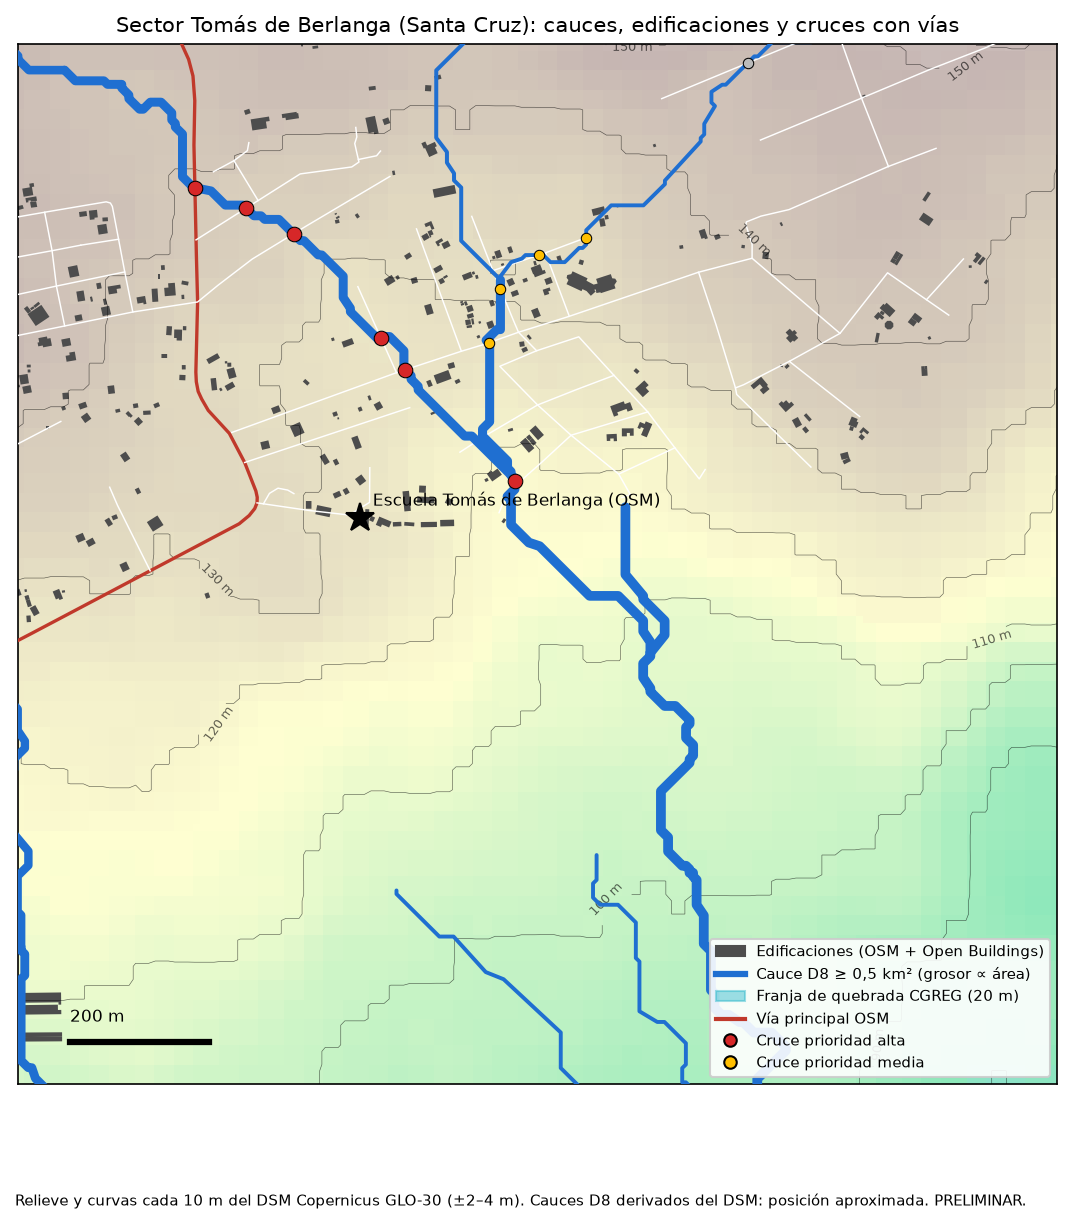
\includegraphics[width=0.78\linewidth]{f_tomas_de_berlanga.png}
  \caption{Sector Tomás de Berlanga (Santa Cruz): cauces D8 de $\geq 0{,}5$~\kmc{} (grosor según el área), edificaciones de OSM y Open Buildings, vías de OSM, franja de quebrada del CGREG y cruces de prioridad alta y media. Relieve y curvas cada 10~m del DSM ($\pm 2$--4~m). Los cauces son modelo y su posición es aproximada.}
  \label{fig:tdb}
\end{figure}

\subsection{Cruces de quebradas con vías}
La tabla~\ref{tab:cruces} resume el inventario de las dos islas. En Santa Cruz, el 91\,\% de los cruces se identifica solo con el cauce D8: casi todos están sobre cauces que no figuran en la cartografía. \textbf{Solo 2 de 687 cruces tienen una estructura cartografiada} (un puente del IGM en la Troncal Insular y una pasarela peatonal de OSM), y OSM no registra ninguna alcantarilla en la isla. San Cristóbal está mejor cartografiado: 123 cruces tocan una quebrada del IGM o de OSM y 11 tienen estructura (7 puentes del IGM, 2 puentes y 2 alcantarillas de OSM).

\begin{table}[ht]
  \centering\small
  \caption{Inventario de cruces quebrada--vía (\texttt{16\_cruces\_quebradas\_vias.py}).}
  \label{tab:cruces}
  \begin{tabular}{lrr}
    \toprule
    & Santa Cruz & San Cristóbal \\
    \midrule
    Intersecciones vía $\times$ cauce & 1\,410 & 721 \\
    Cruces tras agrupar a 40~m & 687 & 325 \\
    \quad prioridad alta / media / baja & 97 / 307 / 283 & 25 / 147 / 153 \\
    \quad de prioridad alta en zona poblada & 88 & 24 \\
    Cruces con estructura cartografiada & 2 & 11 \\
    \bottomrule
  \end{tabular}
\end{table}

Lo que se lee en los cruces de prioridad alta:
\begin{itemize}
  \item \textbf{El eje de La Cascada} (43--44~\kmc) es, con diferencia, el de mayor caudal: una salida sin cauce que cruza 12 calles hasta la Av. Charles Darwin, con $Q_{100} \approx 100$~\mcs{} (58--159) y $Q \approx 290$~\mcs{} (210--377) el 30-oct. El análisis hidrológico de La Cascada da 277--368~\mcs{} para el 30-oct: la concordancia es razonable, aunque el área supera con mucho el rango de validez del método racional.
  \item \textbf{La carretera Puerto Ayora--Baltra cruza 75 cauces.} Ninguno de sus 8 cruces de mayor caudal (16--47~\mcs{} con 100~mm; 46--134~\mcs{} el 30-oct) tiene una estructura cartografiada. Es la única conexión entre el puerto, la parte alta y el aeropuerto.
  \item \textbf{En la parte alta de Santa Cruz}, cauces de 7--10~\kmc{} sin cartografiar cortan tramas de calles sin nombre en Tomás de Berlanga, Miramar, El Bosque y Bellavista (20--26~\mcs{} con 100~mm).
  \item \textbf{En San Cristóbal}, la encañada Galápagos (Barrio Frío) concentra los cruces de mayor caudal ($Q_{100}$ de 25--28~\mcs) y casi todas las estructuras. La vía Puerto Baquerizo Moreno--El Progreso cruza un afluente de 6,5~\kmc{} ($Q_{100} \approx 18$~\mcs) sin estructura cartografiada.
\end{itemize}
Como referencia de capacidad, un tubo de 1~m de diámetro conduce del orden de 1--3~\mcs{} y un cajón de $2 \times 2$~m, unos 10--15~\mcs. \enquote{Ninguna estructura cartografiada} no quiere decir que no haya alcantarilla: falta el inventario de campo (\issue{33}).

\subsection{San Cristóbal: encañadas de Puerto Baquerizo Moreno}
Puerto Baquerizo Moreno recibe el agua de \textbf{11,1~\kmc} (11,5~\kmc{} sin quemar las quebradas); solo el 0,6\,\% de esa área depende del relleno de depresiones de más de 1~m. Llegan 14 quebradas de $\geq 0{,}05$~\kmc, y las cinco mayores suman el 81\,\% del área (tabla~\ref{tab:llegadas}). De 24 vasos de más de 300~\mtres{} en las zonas pobladas o a menos de 100~m, solo 5 son robustos, y \textbf{ninguno está en Puerto Baquerizo Moreno}: allí todos tienen 0,3--0,85~m y desaparecen con el proxy de suelo. A diferencia de La Cascada, el agua no se acumula: atraviesa la ciudad. Los vasos robustos están en El Progreso, en una meseta a ${\approx}\,300$--320~m, a menos de 250~m de dos inundaciones registradas por la SNGR (2021 y 2024).

\begin{table}[ht]
  \centering\small
  \caption{Llegadas principales a las zonas pobladas de San Cristóbal (D8). $Q_{100}$: tormenta tipo II de 100~mm; valor central con CN 70 y $t_c$ de Témez; entre paréntesis, de CN 60 con Témez a CN 80 con Kirpich. Nombres según la correspondencia con el plan de la UGR, que es una hipótesis.}
  \label{tab:llegadas}
  \begin{tabularx}{\linewidth}{l>{\raggedright\arraybackslash}Xrrrr}
    \toprule
    Id & Encañada & $A$ (\kmc) & Cauce: $L$ (km) / $J$ & $t_c$ (h) & $Q_{100}$ (\mcs) \\
    \midrule
    PBM-L01 & Galápagos / Barrio Frío & 5,4 & 8,9 / 4,8\,\% & 1,0--4,2 & 11 (5--35) \\
    PBM-L02 & La Planada $\to$ Manzanillo--El Manantial & 1,8 & 3,7 / 5,3\,\% & 0,4--2,3 & 6 (3--19) \\
    PBM-L03 & Divino Niño & 1,0 & 2,2 / 4,6\,\% & 0,2--1,7 & 4 (2--13) \\
    PBM-L04 & Alejandro Alvear & 0,45 & 1,7 / 5,6\,\% & 0,1--1,2 & 2 (1--7) \\
    PBM-L05 & Playa Mann (quebrada del campus) & 0,31 & 1,3 / 4,6\,\% & 0,1--1,0 & 2 (1--5) \\
    PBM-S01 & Galápagos, salida en Barrio Frío & 10,6 & 11,7 / -- & 1,5--3,5 & 19 (9--58) \\
    \bottomrule
  \end{tabularx}
\end{table}

La ocupación de los cauces es desigual (figura~\ref{fig:pbm}). En conjunto, 228 edificios y unas 550 personas están a $\leq 30$~m de algún sistema de cauce. \textbf{Divino Niño} es el más ocupado en relación con su tamaño: con 1--1,6~\kmc{} y unos 5~\mcs, tiene 14--16 edificaciones sobre la línea del cauce, unas 60 a menos de 15~m y ninguno de sus 7 cruces con estructura cartografiada; desemboca en Playa de Oro, cuya boca, según la UGR, estaba tapada. La franja de 20~m del CGREG cubre el 52--90\,\% de la Galápagos a $\leq 30$~m, el 17--41\,\% de Divino Niño (y termina unos 200~m antes del mar) y nada de Alvear, Playa Mann, Manzanillo--El Manantial ni La Planada. Solo la salida de Barrio Frío tiene cauce cartografiado en su tramo final.

El ranking de puntos sitúa primero la entrada este de la Galápagos (PBM-L01, 8 puntos, 110 edificios en la franja de 20~m), luego la boca de Barrio Frío (PBM-S01, 7), la boca de Divino Niño en Playa de Oro (PBM-S02, 7), la llegada de La Planada (PBM-L02, 6) y la de Divino Niño (PBM-L03, 6). El primer punto de El Progreso es el vaso V03 (puesto 13). El ranking no puntúa los tramos urbanos entre entrada y boca.

\begin{figure}[t]
  \centering
  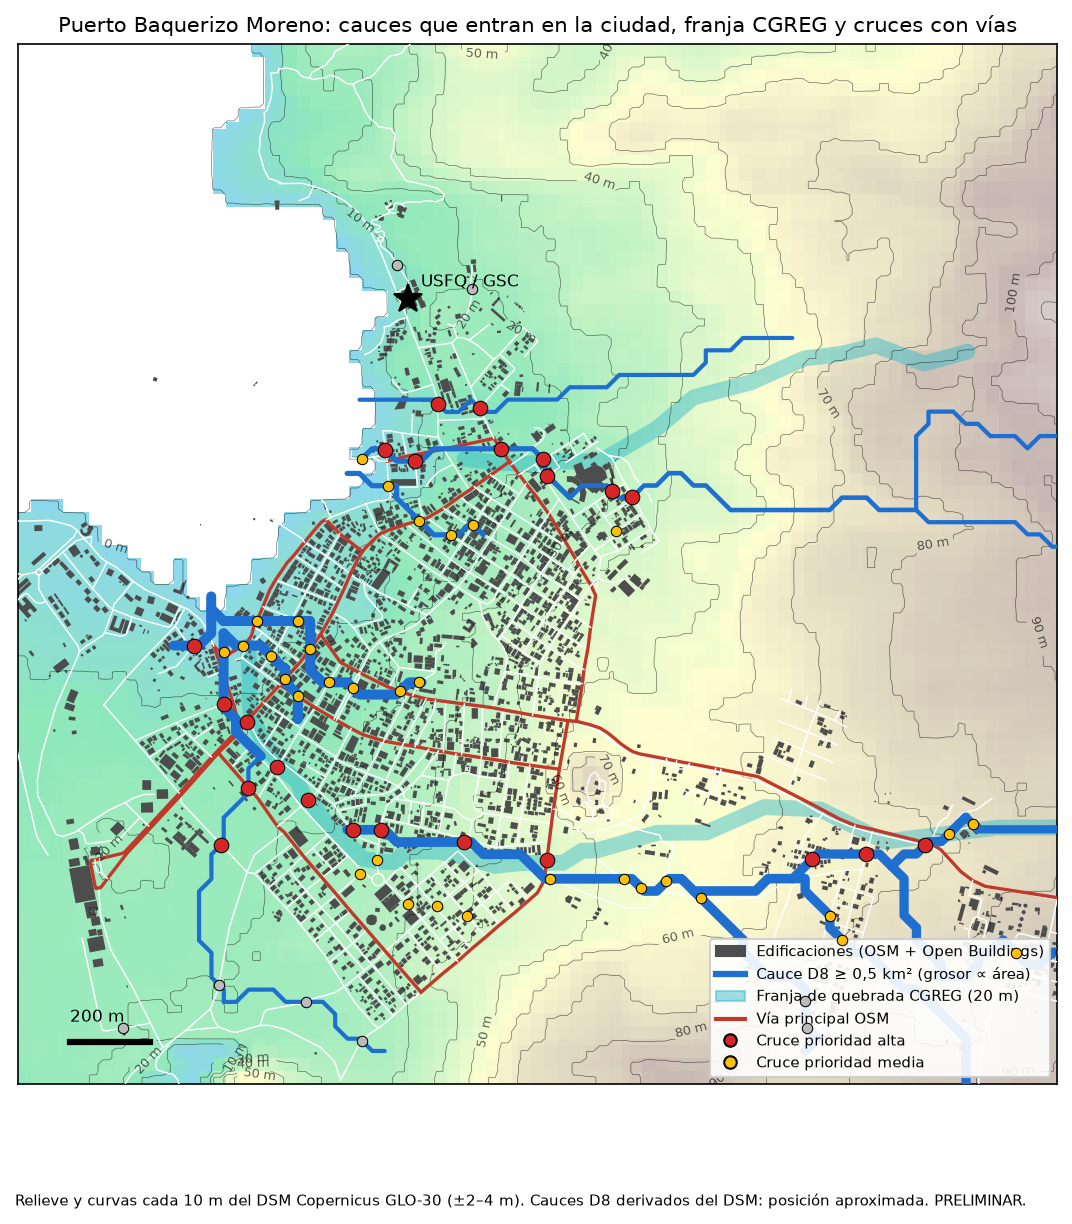
\includegraphics[width=0.78\linewidth]{f_urbano_pbm.png}
  \caption{Puerto Baquerizo Moreno: cauces D8 que entran en la ciudad (grosor según el área), franja de quebrada de 20~m del CGREG (oficial), edificaciones y cruces de prioridad alta y media. Relieve y curvas del DSM ($\pm 2$--4~m). Los cauces son modelo.}
  \label{fig:pbm}
\end{figure}

\subsection{El Plan de Acción de la UGR frente al análisis}
El plan \citep{ugr2026} nombra 47 lugares. Se ubicaron 31 (confianza alta en 13, media en 12 y baja en 6); 16 no figuran en ninguna fuente, 9 de ellos en Puerto Baquerizo Moreno, entre ellos La Picada y los barrios San Francisco y Fragata (\issue{53}). La figura~\ref{fig:ugr} muestra los ubicados.
\begin{itemize}
  \item \textbf{Coincidencia en los ejes.} Los sectores de máxima prioridad del plan se agrupan en torno a cuatro encañadas del análisis: Galápagos, Divino Niño, La Planada $\to$ Manzanillo--El Manantial y Alvear--Playa Mann. La correspondencia de nombres es de confianza alta para Galápagos y la salida de Divino Niño, media para Alvear, Playa Mann y La Planada, y baja para las demás.
  \item \textbf{La franja del CGREG casi no cubre los sectores prioritarios.} Solo toca, en parte, 5 de los 12 lugares contados, todos sobre la Galápagos o junto al hospital.
  \item \textbf{Zanja de 1\,040~m en Manzanillo.} Hay dos hipótesis sobre su cauce: el ramal Manzanillo--El Manantial (${\approx}\,1{,}8$~\kmc; ${\approx}\,6$~\mcs{} con 100~mm) o la Galápagos en su tramo alto (8--9~\kmc; ${\approx}\,24$~\mcs). Con el cauce equivocado, la sección quedaría cuatro veces corta o sobrada (\issue{55}). En ambos casos el agua acabaría en Barrio Frío.
\end{itemize}

\textbf{Desborde lateral Galápagos $\to$ Divino Niño.} Fuera de la franja costera, el cauce de la Galápagos pasa a 466~m del ramal sur de Divino Niño, y en la recta entre ambos el DSM sube solo \textbf{1,2~m} sobre el lecho de la Galápagos (tabla~\ref{tab:bif}). Es menos que el error del DSM. El modelo 2D da allí 0,65~m de calado con la tormenta de Santa Cruz trasladada y 0,28~m con 100~mm; con trazadores, solo el 0,03\,\% del agua de la Galápagos llega a Playa de Oro, frente al 67\,\% que sale por Barrio Frío. Los modelos no reproducen la bifurcación, pero no la descartan: es una \textbf{hipótesis de confianza media-baja y consecuencia alta}, que depende de obstrucciones o rellenos que el DSM no ve (\issue{54}).

\begin{table}[ht]
  \centering\small
  \caption{Desborde lateral entre encañadas de Puerto Baquerizo Moreno (fuera de la franja costera de 200~m). Resalte: lo que sube el DSM sobre el lecho del cauce de origen en la recta hasta el de destino. Cotas del DSM, orientativas.}
  \label{tab:bif}
  \begin{tabular}{lrrr}
    \toprule
    Origen $\to$ destino & Distancia (m) & Resalte (m) & Calado 2D en origen (m) \\
    \midrule
    Galápagos $\to$ Divino Niño & 466 & 1,2 & 0,28 / 0,65 \\
    Galápagos $\to$ Alvear & 876 & 4,0 & 0,27 / 1,05 \\
    Divino Niño $\to$ Alvear & 120 & 2,5 & 0,17 / 0,45 \\
    \bottomrule
  \end{tabular}
  \par\vspace{3pt}\raggedright\footnotesize Calado del modelo 2D (informe 2026-06): tormenta de 100~mm / tormenta de Los Guayabillos trasladada con malla de 15~m.
\end{table}

\begin{figure}[t]
  \centering
  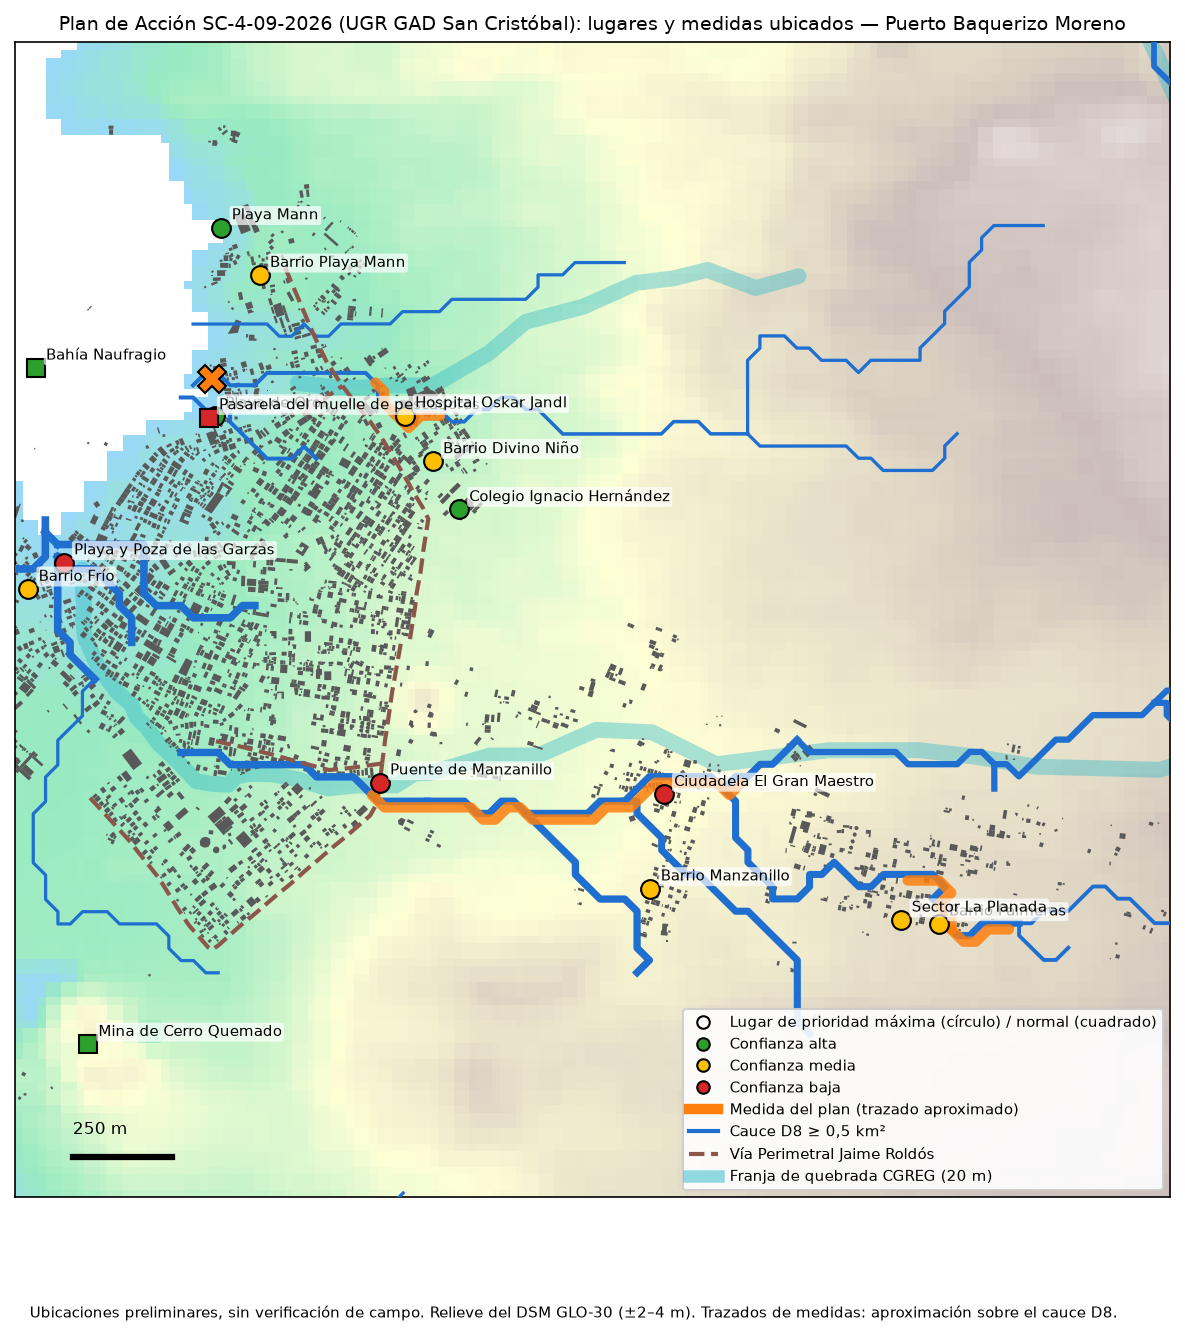
\includegraphics[width=0.74\linewidth]{f_plan_ugr.png}
  \caption{Lugares y medidas del Plan de Acción SC-4-09-2026 (UGR del GAD San Cristóbal) ubicados en Puerto Baquerizo Moreno, con su confianza de ubicación, sobre los cauces D8 y la franja del CGREG. Ubicaciones preliminares, sin verificación de campo; los trazados de las medidas son aproximaciones sobre el cauce D8.}
  \label{fig:ugr}
\end{figure}

\subsection{La quebrada del campus USFQ / GSC}
Una quebrada de unos 0,3~\kmc{} (Playa Mann en el plan) baja de una ladera casi sin edificar, no tiene franja de protección y cruza la Vía Universidad sin paso conocido (figura~\ref{fig:campus}). En un rellano a ${\approx}\,20$~m, a 160--200~m al este del campus, el trazado se vuelve ambiguo: en la rejilla UTM gira al sur hacia Alvear y pasa a 157~m del campus; en la rejilla geográfica original lo atraviesa. Los edificios del campus están 8--13~m más bajos que el rellano, y el resalte en el transecto hacia el GSC es de solo 1,6~m.

El Monte Carlo cuantifica esa ambigüedad (tabla~\ref{tab:mc}): entre el \textbf{12 y el 23\,\%} de las realizaciones cruzan el campus, casi siempre por la esquina noreste, junto a la Vía Universidad. Con 100~mm, el caudal pico de la quebrada en el rellano es de 1,7--3,0~\mcs{} (CN 70) y varía unas 7 veces en la desembocadura (2,0--13,7~\mcs) según el CN y el método de $t_c$. El modelo 2D da con la tormenta trasladada un desborde somero, con una lámina de 2--5~cm en el campus, pero subestima unas 10 veces el caudal de esta quebrada. El resultado \textbf{no es concluyente}: lo que decide es la cota del rellano y de la vía y la existencia de un paso bajo ella (\issue{58}).

\begin{table}[ht]
  \centering\small
  \caption{Monte Carlo del trazado de la quebrada del campus: 100 realizaciones por escenario con ruido gaussiano en el DSM.}
  \label{tab:mc}
  \begin{tabular}{lcc}
    \toprule
    Escenario de ruido & Fracción que cruza el campus & Desembocadura más frecuente \\
    \midrule
    $\sigma = 1$~m, correlación 60~m & 21\,\% & boca D8 de Alvear (66 de 100) \\
    $\sigma = 2$~m, sin correlación & 12\,\% & boca D8 de Alvear (27 de 100) \\
    $\sigma = 2$~m, correlación 60~m & 21\,\% & boca D8 de Alvear (54 de 100) \\
    $\sigma = 3$~m, correlación 60~m & 23\,\% & boca D8 de Alvear (32 de 100) \\
    \bottomrule
  \end{tabular}
\end{table}

\begin{figure}[t]
  \centering
  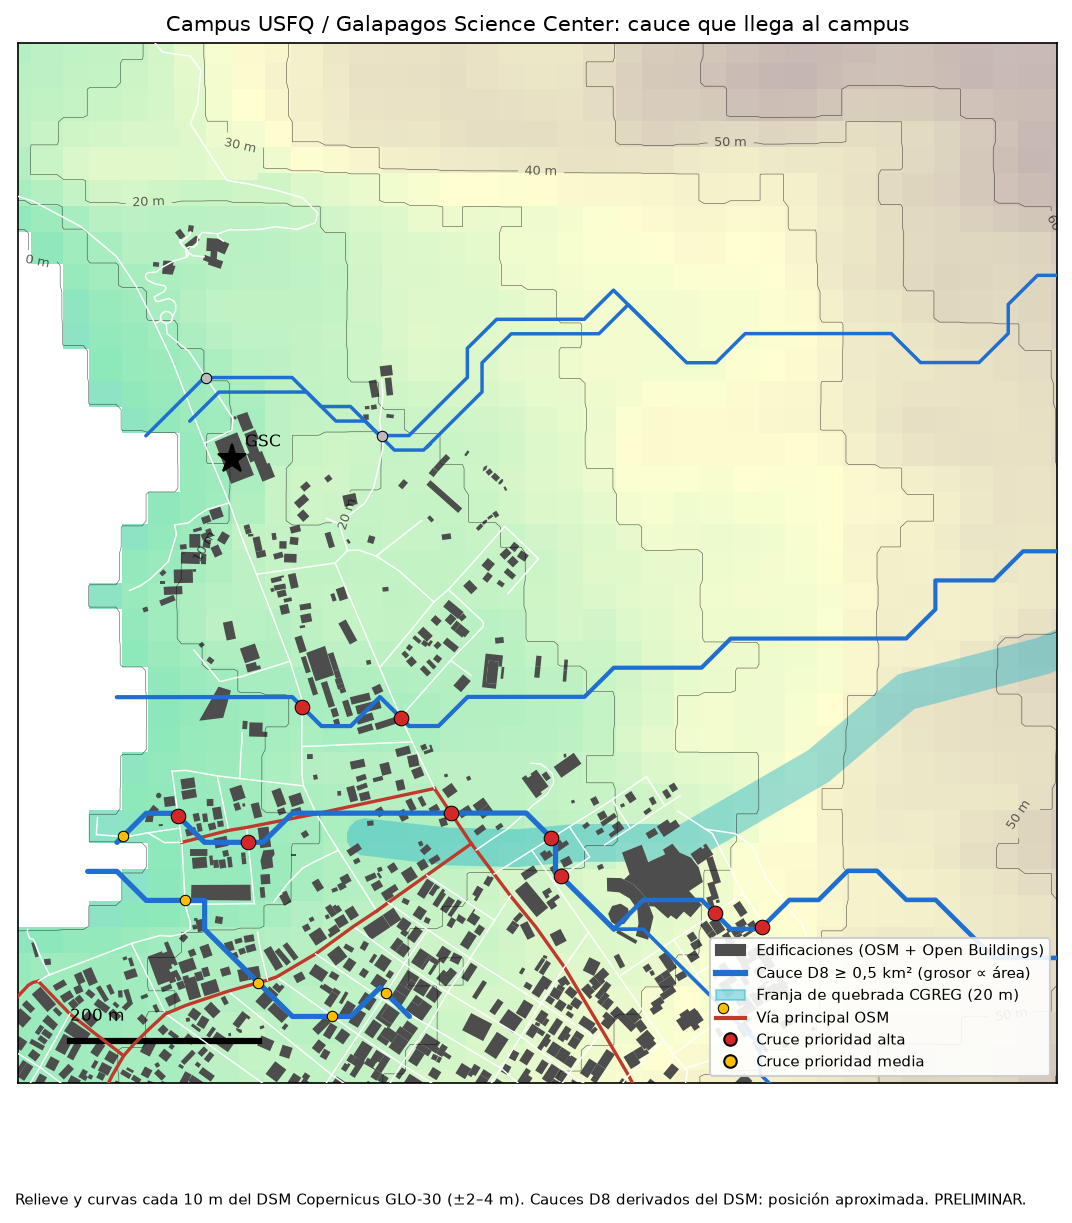
\includegraphics[width=0.7\linewidth]{f_campus_gsc.png}
  \caption{Campus USFQ / Galapagos Science Center: cauce D8 que llega al campus (0,3~\kmc), cauces vecinos, edificaciones y cruces. Relieve y curvas del DSM ($\pm 2$--4~m). El trazado en el rellano es incierto (tabla~\ref{tab:mc}).}
  \label{fig:campus}
\end{figure}

\subsection{Tomas de agua de San Cristóbal}
Se localizaron cuatro tomas principales, ninguna verificada en campo: Cerro Gato (27~l/s; confianza media), Los Americanos (19~l/s; media, desde la coordenada de un registro de la SNGR), La Toma (planta El Progreso; alta) y el manantial El Chino (20~l/s; media) \citep{cgreg2015agua}. Las cotas no coinciden con las de la USFQ: 164 y 150~m frente a ${\approx}\,267$ y ${\approx}\,500$~m del DSM para Cerro Gato y La Toma (\issue{60}). Casi ninguna toma cae sobre un cauce del DSM: en cinco de ellas la cuenca en el punto es de 0,003--0,03~\kmc. O son manantiales de ladera, o la coordenada está desplazada; en ambos casos la escorrentía que llega a la obra es la de la cañada contigua, a 88--224~m.

\begin{table}[ht]
  \centering\small
  \caption{Cuencas de captación de las tomas (propia o cañada contigua, marcada con *) e índice de turbidez y arrastre (0--8). $Q$ con 100~mm, AMC II, rango Témez--Kirpich.}
  \label{tab:tomas}
  \begin{tabular}{lrrrrc}
    \toprule
    Toma & $A$ (\kmc) & Pendiente & Caminos (km) & $Q_{100}$ (\mcs) & Índice \\
    \midrule
    AG-01 Cerro Gato* & 0,60 & 27\,\% & 0 & 4,7--9,2 & 6 (alta) \\
    AG-02 Los Americanos* & 0,62 & 23\,\% & 0,5 & 5,1--9,8 & 8 (alta) \\
    AG-03 La Toma* & 1,26 & 14\,\% & 3,8 & 7,4--14 & 7 (alta) \\
    AG-04 El Chino & 4,75 & 18\,\% & 14,6 & 16--31 & 7 (alta) \\
    AG-10 (FCD)* & 2,87 & 12\,\% & 8,5 & 11--20 & 7 (alta) \\
    AG-09 (FCD) & 0,13 & 20\,\% & 0 & 1,8--2,5 & 4 (media) \\
    AG-11 (FCD)* & 0,16 & 10\,\% & 0 & 1,7--2,7 & 4 (media) \\
    \bottomrule
  \end{tabular}
\end{table}

Las crecidas de esas cuencas (5--30~\mcs{} con 100~mm, y 50--60~\mcs{} en El Chino con suelo húmedo o con la tormenta trasladada) son \textbf{entre 200 y más de 1\,000 veces} lo que se capta, y llegan en 10--60~min. Una toma de cañada con una represa pequeña no puede dejar pasar esa crecida limpia. El modo de fallo esperable es el que ya ocurrió el 15 de abril de 2023, cuando un aluvión arrastró lodo y vegetación y obstruyó una válvula de la represa de Los Americanos: 21 días de emergencia del agua potable y 112 familias (325 personas) afectadas indirectamente \citep{sngr2023}. El índice (tabla~\ref{tab:tomas}) clasifica cinco cuencas en riesgo alto, por pendiente, uso agrícola, caminos y caudal. La red que baja al puerto discurre 1,45~km dentro del polígono de flujos de lodo del CGREG, junto a la Galápagos, y la línea de Cerro Gato cruza 42 cauces (figura~\ref{fig:tomas}).

\begin{figure}[t]
  \centering
  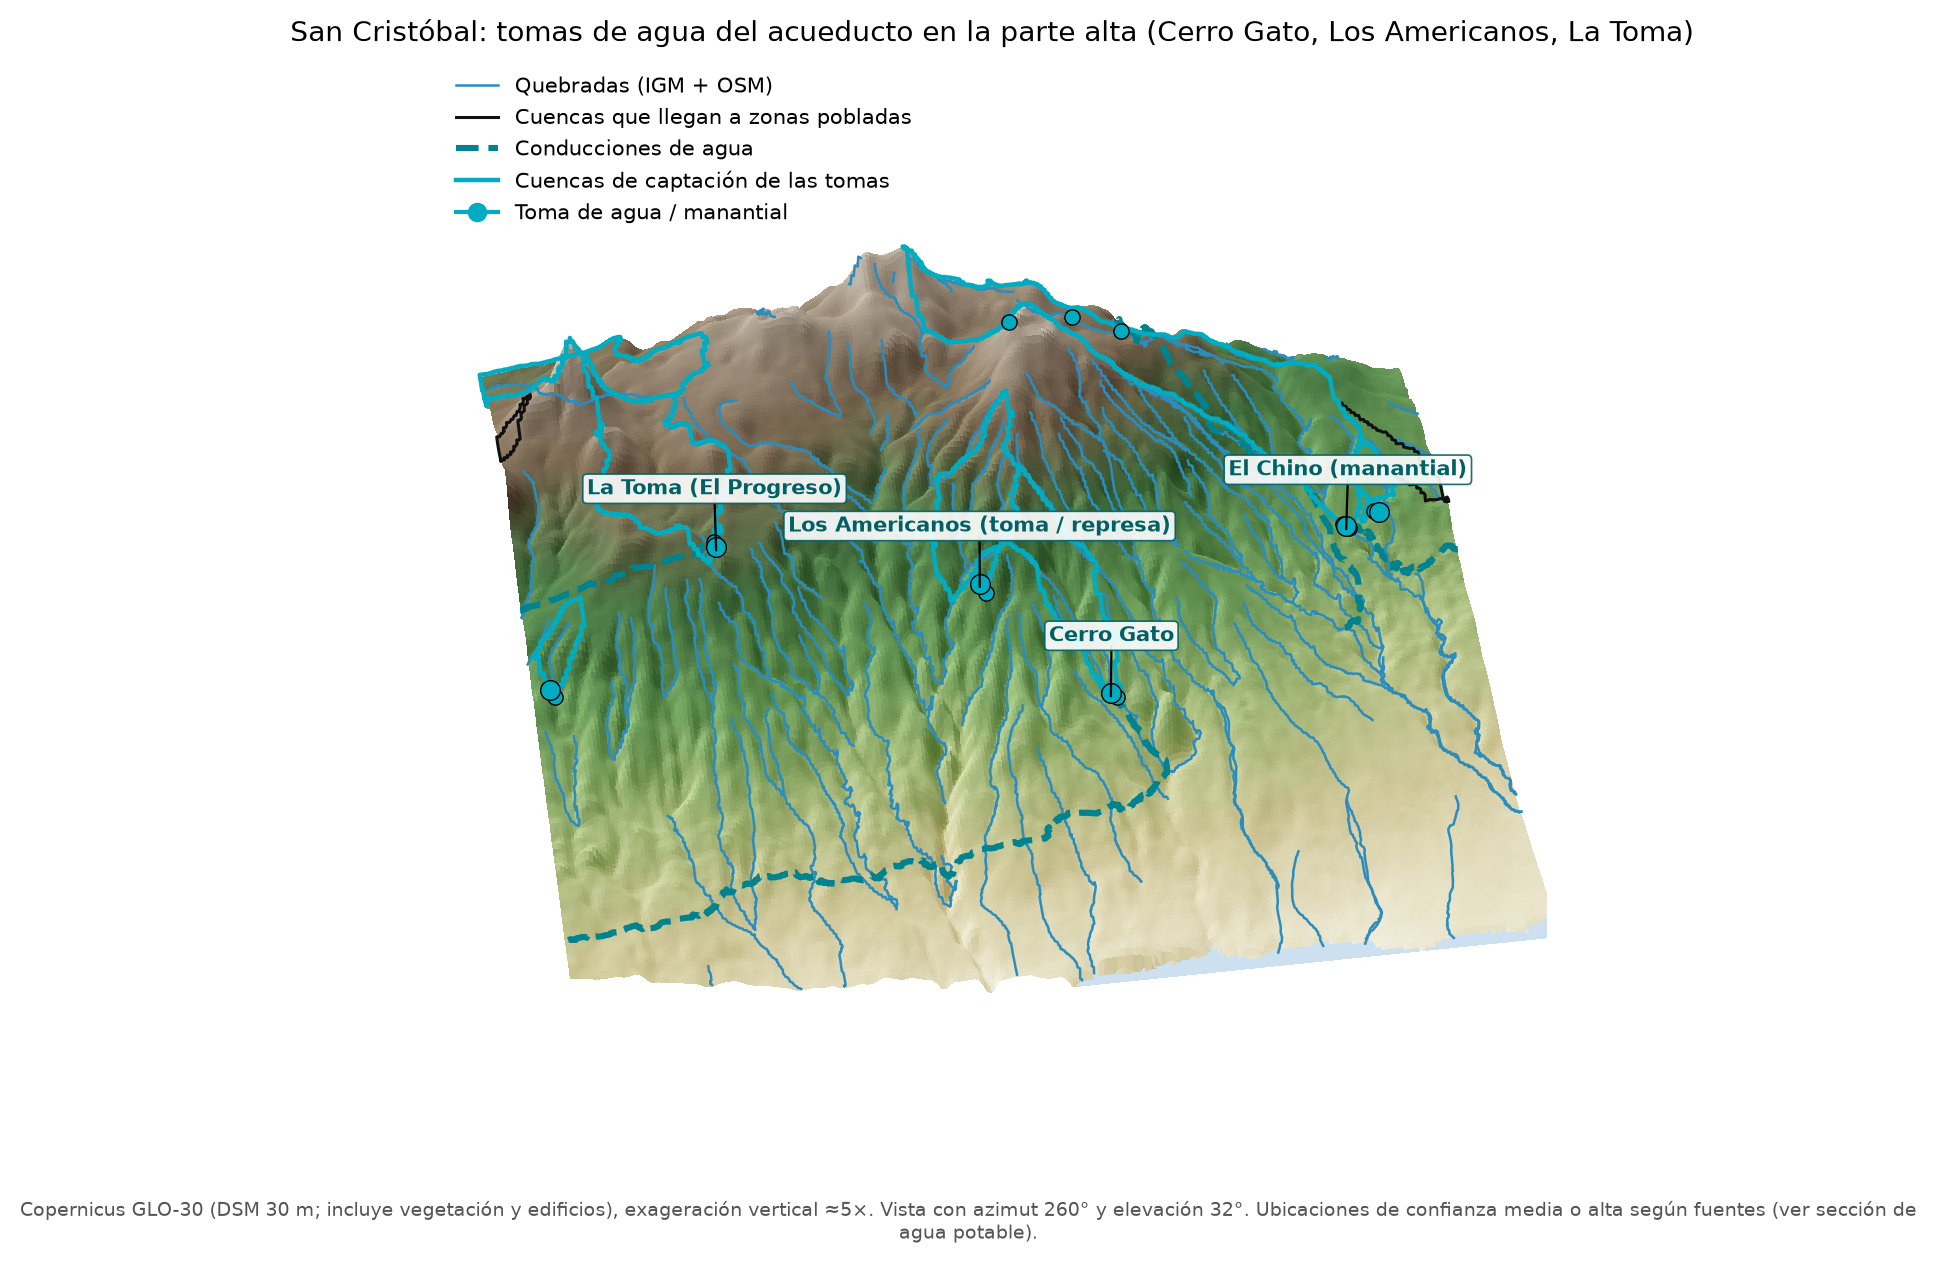
\includegraphics[width=0.85\linewidth]{3d_tomas_agua.png}
  \caption{Vista 3D de la parte alta de San Cristóbal con las tomas de agua (Cerro Gato, Los Americanos, La Toma y el manantial El Chino), sus cuencas de captación, las conducciones del IGM y las quebradas. DSM Copernicus GLO-30 con exageración vertical de $\times 5$. Ubicaciones de confianza media o alta según las fuentes, sin verificación de campo.}
  \label{fig:tomas}
\end{figure}

\subsection{Floreana (exploratorio)}
Tres cauces D8 llegan a la costa de Puerto Velasco Ibarra: el central, que desemboca en Playa Negra (2,07~\kmc), uno norte (1,75~\kmc) y uno sur (4,23~\kmc), a 690~m a cada lado. Hacia el norte hay conexiones coherentes con el terreno: un canal de 240--270~m, a ${\approx}\,68$--72~m de cota, desviaría 1,18~\kmc{} (el 57\,\% de la cuenca de Playa Negra) con una pendiente de 0,5--1,9\,\% y cortes de $\leq 1{,}1$~m. Pero el desnivel (1,3--5,1~m) es del orden del error del DSM, y el agua iría a otra playa cuyo cauce no se conoce. Hacia el sur, una conexión de 500~m solo es posible en la cabecera y desviaría el 4\,\% de la cuenca. Si la cañada La Varonesa/Lobería del plan es el cauce sur, la conexión descrita es justamente la que el terreno no respalda. El veredicto es \textbf{condicional} (\issue{69}).

% =====================================================================
\section{Discusión y limitaciones}

El reconocimiento cumple su objetivo: ordena dónde mirar primero y saca a la luz cauces que la cartografía no tiene, como el de Tomás de Berlanga o los que cruzan la carretera Puerto Ayora--Baltra. Sus cifras deben leerse con estas limitaciones:
\begin{itemize}
  \item \textbf{Ningún punto se ha visitado.} No hay marcas de agua, aforos ni inventario de alcantarillas (\issue{9}, \issue{33}, \issue{5}). Los registros de la SNGR y del plan son datos reportados, con ubicaciones a veces genéricas.
  \item \textbf{El DSM.} Su sesgo frente al IGM es de unos $-2$~m en Puerto Ayora y de $+1{,}5$~m en Puerto Baquerizo Moreno; con RMSE de 3--5~m, los vasos urbanos de 1--2~m pueden ser artefactos de techos o vegetación, y en tramos con un 1--3\,\% de pendiente el trazado de un cauce es incierto en decenas a cientos de metros. El DSM no ve alcantarillas, cauces entubados ni bordillos.
  \item \textbf{Caudales.} Son de modelos agregados sin calibrar, con CN supuestos. En el método racional, el $C$ volumétrico sobre la intensidad pico \textbf{subestima} el caudal (hasta unas 2 veces), y por encima de 10--25~\kmc{} la cifra es solo una escala. La lluvia de una estación se aplica a toda la isla, sin reducción areal, y en San Cristóbal no hay lluvia medida en las cuencas urbanas.
  \item \textbf{Métodos que no concuerdan.} Para la quebrada del campus, el racional da ${\approx}\,1$~\mcs{} con 100~mm, la tormenta tipo II 1,7--3,0~\mcs{} y el modelo 2D 0,2~\mcs. La diferencia con el 2D viene de que este llena primero las microdepresiones del DSM. La dispersión es una medida honesta de la incertidumbre.
  \item \textbf{Rankings.} Sus pesos son convencionales y no se calibraron; sirven para ordenar inspecciones, no para comparar riesgos.
  \item \textbf{Floreana} es exploratorio y de confianza baja: solo DSM, sin cartografía de las cañadas y sin nombres asignados.
  \item \textbf{Plan de la UGR.} Es interno y no se reproduce; 16 de sus lugares no se ubicaron y la correspondencia de nombres es una hipótesis.
\end{itemize}

% =====================================================================
\section{Conclusiones y trabajo futuro}
\begin{enumerate}
  \item En Santa Cruz hay 120 puntos potenciales de inundación fuera de La Cascada, 10 de prioridad alta. El sector Tomás de Berlanga está atravesado por un cauce de 9,4~\kmc{} sin cartografiar, con un pico estimado de 99--139~\mcs{} el 30-oct, que desemboca en La Cascada.
  \item De 687 cruces quebrada--vía en Santa Cruz, solo 2 tienen una estructura cartografiada; la carretera Puerto Ayora--Baltra cruza 75 cauces. En San Cristóbal hay 325 cruces, 11 con estructura.
  \item En Puerto Baquerizo Moreno el riesgo es el paso del agua, no su acumulación: ningún vaso urbano es robusto. Divino Niño es la cañada más ocupada en relación con su tamaño, y el terreno admite, sin demostrarlo, un desborde de la Galápagos hacia ella.
  \item La entrada de la quebrada de Playa Mann al campus de la USFQ es plausible (12--23\,\% de los trazados Monte Carlo), pero no concluyente.
  \item Las tomas de agua de San Cristóbal están expuestas a crecidas cientos de veces mayores que lo captado; el fallo esperable es la colmatación, como en abril de 2023.
\end{enumerate}

Los datos que cambiarían estas conclusiones son:
\begin{itemize}
  \item el inventario de campo de cruces y alcantarillas, con sección y estado (\issue{33}, \issue{5});
  \item el trazado del cauce, la cota de la escuela y la ruta de evacuación en Tomás de Berlanga (\issue{66});
  \item la cota del rellano y de la Vía Universidad frente al campus, con GNSS (\issue{58}), y la verificación del collado Galápagos--Divino Niño (\issue{54});
  \item la ubicación de los lugares del plan no localizados y el cauce de la zanja de Manzanillo (\issue{53}, \issue{55}, \issue{70});
  \item la ubicación y la cota verificadas de las tomas y conducciones (\issue{60}) y el estado del agua potable tras el evento (\issue{59});
  \item las cañadas de Floreana (\issue{69}), la lluvia medida en la ciudad de San Cristóbal (\issue{61}) y un DTM de $\leq 1$~m en los poblados (\issue{16}).
\end{itemize}

\section*{Disponibilidad de datos y código}
{\small Todo el procesamiento es reproducible desde el repositorio público \emph{mayait/sosgalapagos-datos}, carpeta \texttt{geodatos/}. Varios scripts comparten número (\issue{57}); se citan por su nombre completo:
\begin{itemize}
  \item \texttt{scripts/15\_santa\_cruz\_inundacion.py}: puntos de Santa Cruz y Tomás de Berlanga (\texttt{estudios/santa-cruz/datos/resumen.json}, \texttt{puntos\_inundacion.geojson}, \texttt{vasos.geojson});
  \item \texttt{scripts/16\_cruces\_quebradas\_vias.py}: cruces de ambas islas (\texttt{estudios/*/datos/cruces.csv} y \texttt{.geojson});
  \item \texttt{scripts/16b\_urbano\_sectores.py}: diagnóstico urbano de Tomás de Berlanga y de Puerto Baquerizo Moreno (\texttt{datos/urbano/});
  \item \texttt{scripts/16c\_agua\_san\_cristobal.py} y \texttt{scripts/26\_cuencas\_tomas\_san\_cristobal.py}: tomas, conducciones e índice de turbidez (\texttt{estudios/san-cristobal/datos/agua/});
  \item \texttt{scripts/16d\_plan\_ugr\_sancristobal.py}: lugares del plan de la UGR (\texttt{datos/ugr/});
  \item \texttt{scripts/17\_san\_cristobal\_inundacion.py}: cuencas, vasos, ranking, quebrada del campus, Monte Carlo y contraste con el IGM (\texttt{estudios/san-cristobal/datos/resumen.json});
  \item \texttt{scripts/27\_canadas\_oficiales\_san\_cristobal.py}: correspondencia con las cañadas oficiales y desborde lateral (\texttt{contraste\_plan\_ugr.json});
  \item \texttt{scripts/28\_floreana\_canadas.py}: Floreana (\texttt{datos/floreana/}).
\end{itemize}
Los textos de los estudios están en \texttt{geodatos/estudios/santa-cruz/texto/} y \texttt{geodatos/estudios/san-cristobal/texto/}. Este informe se compila con \texttt{informes/compilar.sh 2026-05-reconocimiento}.\par}

\bibliographystyle{sosg}
\bibliography{referencias,bib-2026-05}

\end{document}
